\documentclass[11pt]{article}
\usepackage[margin=0.85in]{geometry}
\usepackage{amsmath,amssymb,graphicx,hyperref}
\setlength{\parindent}{0pt}\setlength{\parskip}{7pt}
\setlength{\emergencystretch}{3em}
\begin{document}
{\Large Cofactor-pencil reconstruction: recovery and rejection tests}\\
November 13, 2026. Unsigned producer evidence [pcc:unverified].

\textbf{Candidate.} Encode the norm coefficient equations as homogeneous
quadrics $q_t(w)=\sum_{i,j}Q_t(i,j)w_iw_j$ after eliminating the target branch.
Search a small symmetric pencil $S(\lambda)=\sum_t\lambda_t Q_t$ for a
corank-one singular point whose cofactor pairings all vanish.
The higher-dimensional norm-to-pencil bridge is not yet formalized; certificate
completeness and an efficient finder remain unproved. This stage checks
sufficient recovery and exact controls.

\textbf{Checked recovery.} Over any field, let a supplied symmetric $m\times m$ matrix $S$
satisfy $\det S=0$, $\operatorname{rank}S+1=m$, and $\operatorname{adj}S\ne0$.
If
\[
 \langle Q_t,\operatorname{adj}S\rangle
 :=\sum_{i,j} Q_t(i,j)(\operatorname{adj}S)_{ij}=0\quad\text{for every }t,
\]
then a nonzero vector $w$ satisfying every $q_t(w)=0$ exists. Lean proves the
adjugate rank bound, all minor identities and scaled outer-product extraction.
The generic theorem does not assume $S$ belongs to a particular pencil.

Indeed $S\operatorname{adj}S=0$ and the matrix rank inequality force
$\operatorname{rank}(\operatorname{adj}S)\leq1$. Symmetry and the verified
nonzero condition give $\operatorname{adj}S=sww^T$, $s\ne0$.
Every pairing becomes $s q_t(w)=0$. No square root is needed.

\begin{center}
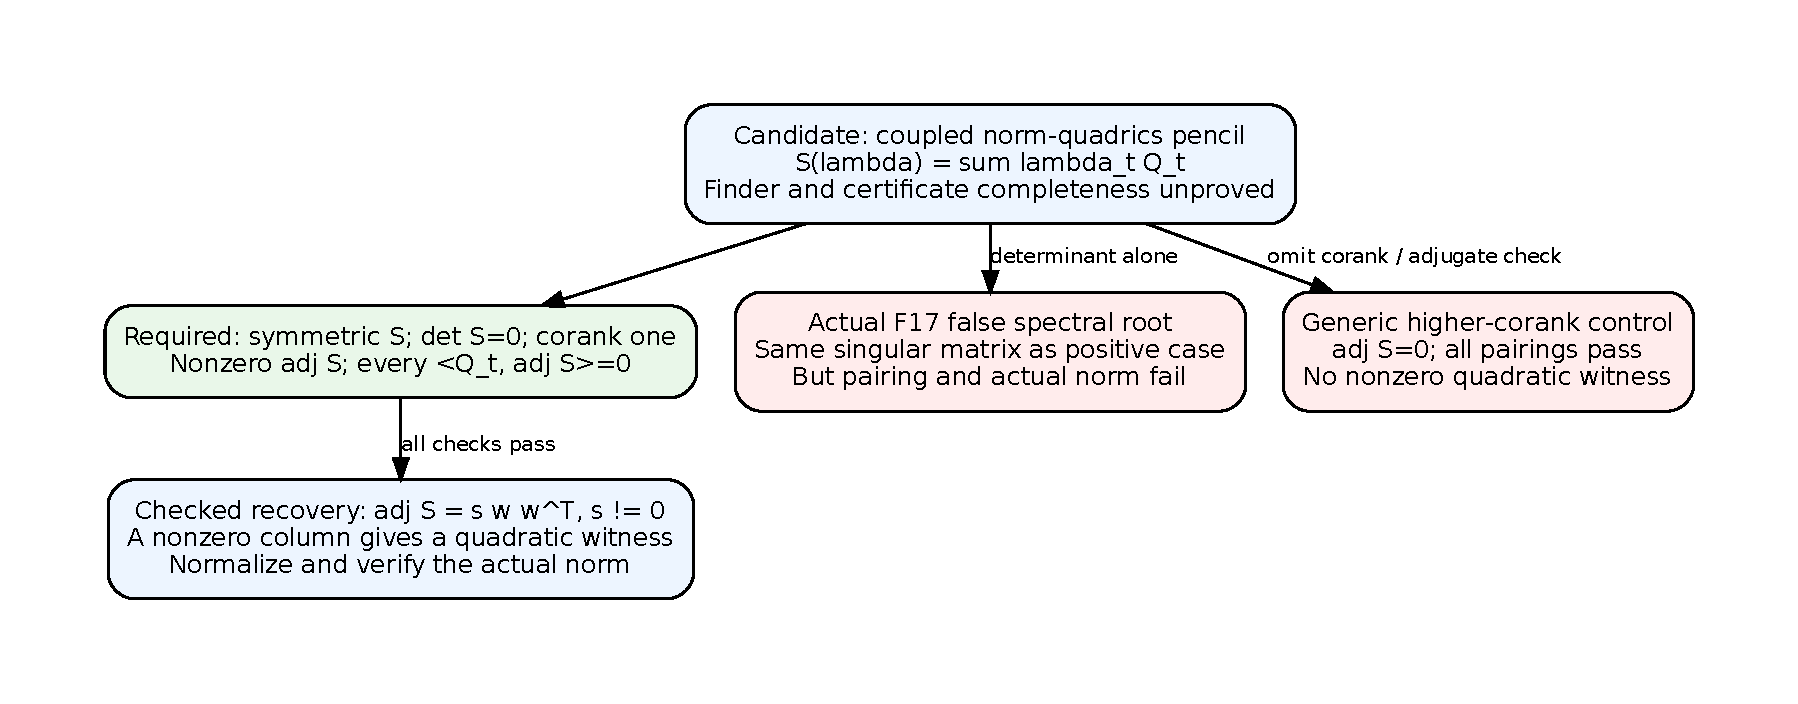
\includegraphics[width=0.97\linewidth,height=0.34\textheight,keepaspectratio]{certificate.pdf}
\end{center}

\newpage
{\Large Actual norm fixture, false positives and evidence}

\textbf{Two-support pencil.} With $w=(v,u)$ after branch elimination,
\[
 Q_1=\begin{pmatrix}1&0\\0&-U\end{pmatrix},\quad
 Q_2=\begin{pmatrix}0&y\\y&-V\end{pmatrix},\quad
 S(a,b)=\begin{pmatrix}a&by\\by&-aU-bV\end{pmatrix}.
\]
Here $U=q+x_1+x_2$ and $V=q^2+\alpha+qU-x_1x_2$ for curve coefficient
$\alpha$. Lean checks
\[
 \det S=-Ua^2-Vab-y^2b^2,\quad
 \langle Q_1,\operatorname{adj}S\rangle=-2Ua-Vb,\quad
 \langle Q_2,\operatorname{adj}S\rangle=-Va-2y^2b.
\]

\textbf{Positive and negative actual-curve controls.} On
$y^2=x^3+2x+2$ over $\mathbb F_{17}$ with supports $(5,1),(6,3)$, use
$(a,b)=(3,1)$. Target $(10,6)$ gives $(U,V)=(4,10)$; target $(0,6)$ gives
$(11,6)$. Both give exactly $S=\left(\begin{smallmatrix}3&6\\6&12\end{smallmatrix}\right)$,
with determinant zero and nonzero adjugate. Its normalized adjugate column
has slope15. Both cofactor tests and the actual positive norm pass.
For the negative target a cofactor test and the actual recovered norm fail.
Thus a determinant root and nonzero adjugate alone are insufficient.

\textbf{Higher-corank control.} In the coordinate-square pencil,
$S=\operatorname{diag}(1,0,0)$ is nonzero singular with zero adjugate.
Every cofactor pairing passes, although $w_i^2=0$ for all $i$ has no nonzero
witness. This is a generic control, not a curve norm instance.

\textbf{Formal scope.} Main theorem: \path{NormDualPencil.recoverQuadratic}.
Exact formulas and all control statements are mapped in the README.
Source \path{71f1bfb22}; build005 passed3147 jobs; tracked-source gate passed62
declarations with zero additional trusted axioms. Earlier declaration hashes
are unchanged. Import-inclusive fresh status is in the evidence directory.
Failed builds and final source hashes are retained; all standing is unsigned.

Native determinant record \path{IDC1h25bf8a5444f4976f} and cofactor record
\path{IDC1h76b1a590e132b252} each have32 statement-derived and32 extra-stream
points and a source hash. They certify expression checks only, not Lean execution
or a search bound.

\textbf{Open obligations.} A general norm-to-pencil completeness/regularity
proof and a constructive finder costing $2^{o(n)}$ bit operations remain absent,
with $n=\lceil\log_2 r\rceil$ for prime subgroup order $r$.
Polynomial determinant evaluation does not find the required cofactor point.
No empirical scaling run, paid compute or performance claim was made.
Sources: pinned Mathlib adjugate/rank declarations and actual norm proofs;
previous kernel/jet scope reviewed. KB unavailable; no novelty asserted.
\end{document}
